\documentclass[12pt]{article}

\usepackage{times}
\usepackage[final]{graphicx}
\usepackage{hyperref}
\usepackage{verbatim}
\usepackage{enumerate}
\usepackage{color}

\setlength{\topmargin}{-0.5in}
\setlength{\oddsidemargin}{0in}
\setlength{\evensidemargin}{0in}
\setlength{\textwidth}{6.5in}
\setlength{\textheight}{9.0in}

\begin{document}

\centerline{\bf \Large CS295/CS395/CSYS395: \href{CS295_395_Syllabus.pdf}{\underline{Evolutionary Robotics}}}

\vspace{0.5cm}

\centerline{\bf \large Programming Assignment 9b of 10}
\vspace{0.25cm} \centerline{\color{red}DRAFT: Port from Bullet to Bullet by Shane Celis \color{black}}
\vspace{0.5cm}

\centerline{\large Assigned: Friday, October 28, 2011}

\vspace{0.5cm}

\centerline{\large Due: Friday, November 4, 2011 by midnight}

\vspace{0.5cm}
\noindent \color{red}CHANGES:  I removed a step that was ODE specific regarding the collision detection.  Step 10 includes instructions for setting parameters for both position control and velocity control.  \color{black}

\noindent \textbf{Description:} In assignment 7 you added eight motors to your robot. In assignment 8, you added four sensors. In this assignment, you will add a randomly-weighted synapse connecting each sensor to each motor. This will cause the robot to exhibit non-random behavior, even though it has a random neural network: each time a foot comes in contact with the ground, the motors will respond in the same way. When you capture five images of the robot using a neural network, your images should show that the robot is no longer moving randomly: as can be seen in Fig. \ref{Fig1}, the robot maintains more or less a similar pose as it moves about.

\begin{figure}
\centerline{
a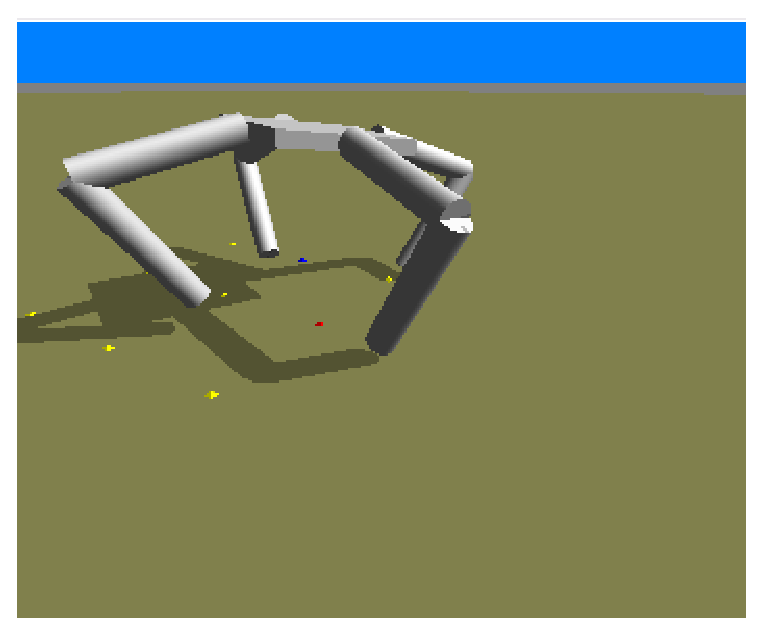
\includegraphics[height=4cm]{Fig1a}
b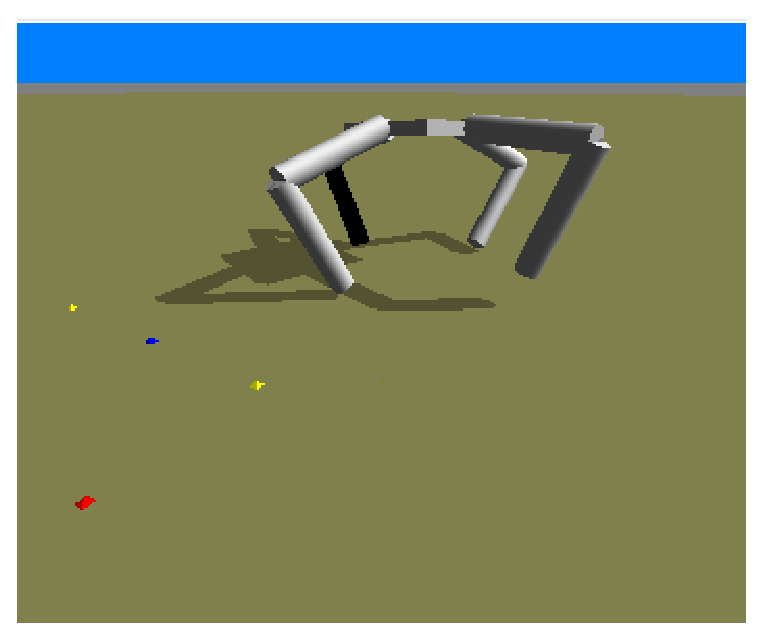
\includegraphics[height=4cm]{Fig1b}
c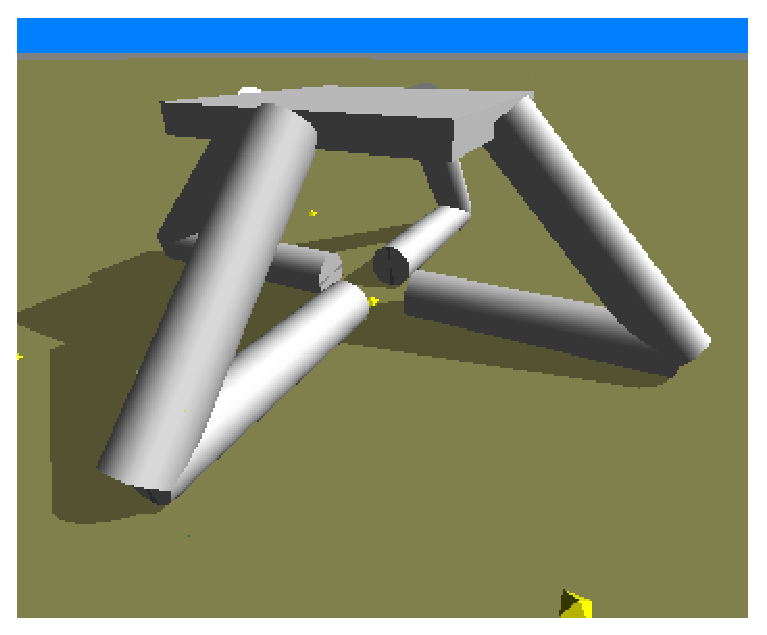
\includegraphics[height=4cm]{Fig1c}}
\centerline{
d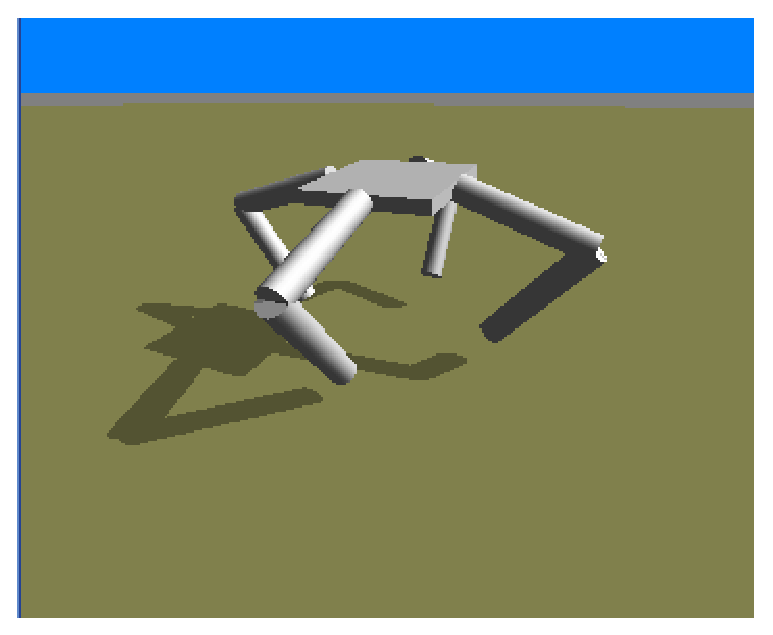
\includegraphics[height=4cm]{Fig1d}
e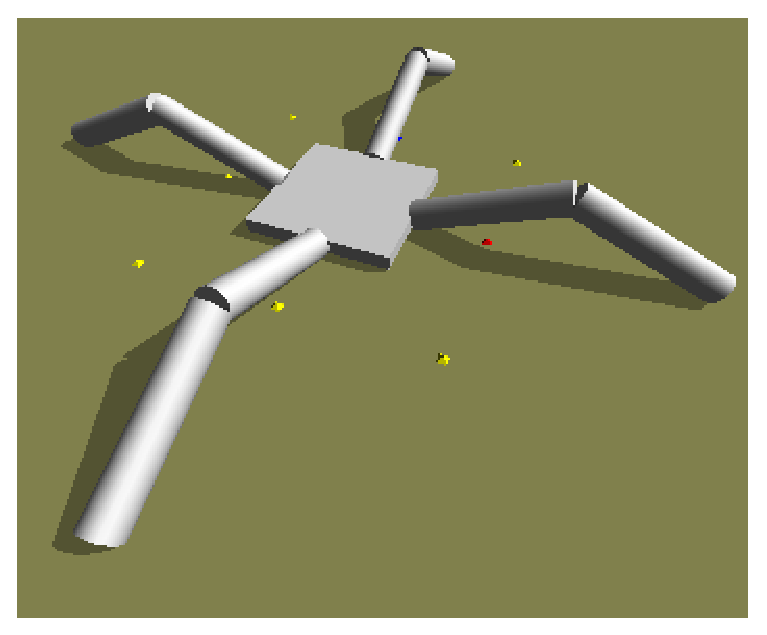
\includegraphics[height=4cm]{Fig1e}}
\caption{Visual display of the robot with randomly-weighted synapses connecting the four touch sensors to the eight motors.}
\label{Fig1}
\end{figure}

\begin{enumerate}

\item Back up Assignment\_8 on a flash drive or another computer so that you can always return to your completed eighth assignment.

\item Copy directory Assignment\_8, which contains your submitted document and the entire Bullet folder. Rename the new directory Assignment\_9.

\item Create a member variable in \verb|RagdollDemo.h| that is a two dimensional array after the \verb|touches| member:\\
    \texttt{double weights[4][8];}

\item At the beginning of the \texttt{initPhysics} method, set each value in the array to a random value in the range $[-1,1]$. You will need to use \texttt{rand()} as you did previously. Now, element \texttt{weights[i][j]} encodes the weight of the synapse connecting touch sensor $i$ to motor $j$.

\item In \texttt{clientMoveAndDisplay}, just before you call \texttt{ActuateJoint(i,motorCommand, ...)} (which sends desired angle \texttt{motorCommand} to motor $i$), you need to set \texttt{motorCommand} based on the values of the sensors, instead of setting it randomly. This is done by creating a \texttt{for} loop that iterates over each of the four sensors before calling \texttt{ActuateJoint()}.

\item During each pass through the loop, the value of that touch sensor is multiplied by the weight of the corresponding synapse, and added to \texttt{motorCommand}.

\item After the loop, you must threshold \texttt{motorCommand} so that it lies in the range $[-1,1]$:\\
    \texttt{motorCommand = tanh(motorCommand);}

\item You must then expand the range of \texttt{motorCommand} so that it can specify desired angles between $[-45^o,45^o]$: \\
    \texttt{motorCommand = motorCommand*45;}

\item Finally, send \texttt{motorCommand} to \texttt{ActuateJoint(...)}.

\item Compile, run and debug your simulation. If you find that your robot moves and then comes to a stop, you may try increasing the speed and force of the motors. Alternatively, you may have to decrease the simulation step size. I found that a max motor force of $40\, N$ worked well for the position control in \verb|ActuateJoint|:

\begin{verbatim}
    void ActuateJoint(int jointIndex, double desiredAngle, double dt) {
      ...
      double maxForce = 40.;
      joints[jointIndex]->enableMotor(true);
      ...
    }
\end{verbatim}

For the velocity control in \verb|ActuateJoint2|, a proportionality constant $k$ of $100\, m/(s^o) $ worked well on my machine: 

\begin{verbatim}
    void ActuateJoint2(int jointIndex, double desiredAngle, double dt) {
      ...
      double k = 100.;
      double maxForce = 40.;
      joints[jointIndex]->enableAngularMotor(true, -k * diff, maxForce*dt);
    }
\end{verbatim}

\item You may also find that the particular synapse weights do not produce motion for different settings of the motor speed, force and simulation time step. You can get your code to produce a different sequence of random numbers by setting the random seed at the very beginning of your code using \texttt{srand(int s)}. So, \texttt{srand(0)} will always produce the same sequence of random numbers every time you run your code, but changing to \texttt{srand(1)} will cause a different sequence of random numbers. Try running your code with different initial random seeds, and you should get different motion patterns, one of which will cause the robot to self-displace as in Fig. \ref{Fig1}.

\item Once you have a self-displacing robot, capture five images from its motion illustrating that it maintains a similar pose, but does move, as in Fig. \ref{Fig1}. Copy them into your document and submit to the T.A.

\end{enumerate}

\end{document} 
